\section{Theoretical background}
    %%% some intro stuff

    \subsection{Resistor-Transistor Logic}
        Resistor-Transistor Logic (RTL) is a fundamental digital logic family extensively used in electronic circuit design. 
        It leverages transistors for logic gates and integrates resistors for biasing and signal conditioning. 
        This straightforward and cost-effective approach to building digital circuits lays the groundwork for advanced logic families and integrated circuits. 

    \subsection{Bipolar Junction Transistor}
        The Bipolar Junction Transistor (BJT) consists of three layers: the emitter, the base, and the collector. 
        N-type and P-type materials, each doped with different impurities, compose these layers. 
        The emitter and collector are doped oppositely, either with excess electrons or holes, while the base remains lightly doped. 
        This setup creates two types of BJTs: NPN and PNP, defined by the arrangement of the layers.
        \begin{figure}[H]
            \centering
            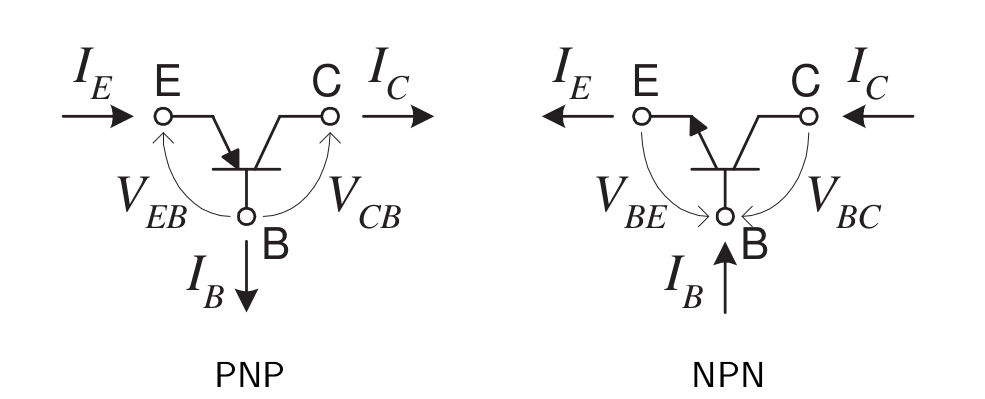
\includegraphics[width=0.7\textwidth]{figures/PNP_NPN.png}
            \caption{PNP and NPN Bipolar Junction Transistors}
            \label{fig:PNP_NPN}
        \end{figure}
        \noindent
        In its off state, the BJT functions as a switch, effectively isolating the collector from the emitter. 
        This behavior is consistent for both NPN and PNP BJTs. During this state, the collector-emitter junction acts as a barrier, preventing any significant current flow, much like a dam restraining water. 
        Additionally, the base-emitter junction remains non-conductive, blocking the flow of current from the emitter to the collector. \\
        Transitioning to the active state, the BJT takes on the role of a signal amplifier. A small current flows from the emitter to the base, giving rise to a more substantial current that courses from the collector to the emitter. 
        This relationship between the base and collector currents forms the cornerstone of the BJT's amplification capability. \\\\
        This amplification phenomenon hinges on the controlled movement of charge carriers across the emitter-base junction. 
        As electrons (or holes) traverse this junction, they engage with the majority carriers in the adjacent layer, resulting in the creation of localized charge regions. 
        These regions facilitate the flow of current from the collector to the emitter. \\
        In the NPN BJT, electrons cross from the emitter to the base. 
        The thinness of the base region and the attractive force exerted by the positively doped collector allow some electrons to overcome the barrier and reach the collector. 
        The modest base current exerts a substantial influence, enabling small variations in its magnitude to produce significant changes in the collector current. \\
        Similarly, the PNP BJT witnesses the flow of holes from the emitter to the base, and the base current governs the larger collector current. 
        In this configuration, the base-emitter junction, now comprised of N-type emitter material and P-type base material, emulates the behavior exhibited by the NPN counterpart. 
        Holes traverse the base region, ultimately converging at the collector, thus amplifying the overall current. \\\\
        As we increase the base current, a point is reached where the collector current can't increase further, regardless of the base current's rise. 
        This state is called saturation. It's as if the BJT switch is turned on fully, allowing maximal current flow through the collector-emitter path. \\
        On the opposite side, as the base current drops, the collector current also decreases until it nearly vanishes. 
        This state is known as cutoff, where the BJT operates as a near-perfect insulator, stopping any significant current from flowing through the collector-emitter junction.
        
    \subsection{Boolean Algebra}        
        Boolean algebra is a fundamental branch of mathematics that deals with binary variables and logical operations, providing a formal framework for analyzing and manipulating logical expressions. 
        Binary variables can take on one of two values: 0 or 1, representing, respectively, false and true. These binary values correspond to the states of a switch, a circuit element, or a logical proposition. \\
        Boolean algebra uses logical operators such as conjunction (and) denoted as $\land$, disjunction (or) denoted as $\lor$, and the negation (not) denoted as $\neg$.
        Boolean algebra is characterized by several key properties that enable the manipulation and simplification of logical expressions. 
        Some of the fundamental properties include: \\

        \textbf{Commutative Property:}
        \begin{align*}
        \text{AND:} \quad & A \land B = B \land A \\
        \text{OR:} \quad & A \lor B = B \lor A
        \end{align*}

        \textbf{Associative Property:}
        \begin{align*}
        \text{AND:} \quad & (A \land B) \land C = A \land (B \land C) \\
        \text{OR:} \quad & (A \lor B) \lor C = A \lor (B \lor C)
        \end{align*}

        \textbf{Distributive Property:}
        \begin{align*}
        \text{AND over OR:} \quad & A \land (B \lor C) = (A \land B) \lor (A \land C) \\
        \text{OR over AND:} \quad & A \lor (B \land C) = (A \lor B) \land (A \lor C)
        \end{align*}

        \textbf{Identity Property:}
        \begin{align*}
        \text{AND:} \quad & A \land 1 = A \\
        \text{OR:} \quad & A \lor 0 = A
        \end{align*}

        \textbf{Complement (Inverse) Property:}
        \begin{align*}
        \text{AND:} \quad & A \land \neg A = 0 \\
        \text{OR:} \quad & A \lor \neg A = 1
        \end{align*}

        \textbf{Double Negation:}
        \[
        \neg(\neg A) = A
        \]